\documentclass{article}
\usepackage[utf8]{inputenc}
\usepackage[parfill]{parskip}

% packages required for tikz and tikzplotlib
\usepackage{pgfplots}
\usepackage{tikz}
\usetikzlibrary{positioning}
\DeclareUnicodeCharacter{2212}{−}
\usepgfplotslibrary{groupplots,dateplot}
\usetikzlibrary{patterns,shapes.arrows}
\pgfplotsset{compat=newest}

% This is for scaling tikzpictures to \textwidth
\usepackage{environ}
\makeatletter
\newsavebox{\measure@tikzpicture}
\NewEnviron{scaletikzpicturetowidth}[1]{%
  \def\tikz@width{#1}%
  \def\tikzscale{1}\begin{lrbox}{\measure@tikzpicture}%
  \BODY
  \end{lrbox}%
  \pgfmathparse{#1/\wd\measure@tikzpicture}%
  \edef\tikzscale{\pgfmathresult}%
  \BODY
}
\makeatother

\begin{document}

\begin{center}
	{\scshape\LARGE 5 Minutes of Fame \par\vspace{5cm}}
	{\LARGE TikZ and tikzplotlib \par\vspace{5cm}}
	{\LARGE by Luca}\newpage
\end{center}

\section{TikZ}
TikZ can be used for creating graphics of different shape, size and complexity, all within your LaTeX source code. Let's start with some simple lines and arrows. \vspace{5mm}

\begin{tikzpicture}

\draw (-1,0) -- (0,1);
\draw [red, thick, ->] (2,0) -- (1,1);
\filldraw[red] (2,0) circle (2pt) node[anchor=north]{vector};
\draw (3,1) .. controls (4,-1) and (6,-1) .. (7,1);

\end{tikzpicture}


You can also use it to draw different geometric shapes: \vspace{5mm}

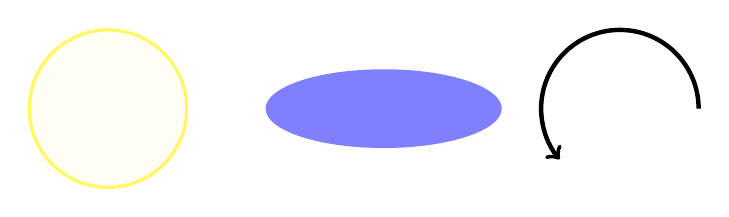
\begin{tikzpicture}

\filldraw[color=yellow!60, fill=yellow!5, very thick](-1,0) circle (1);
\fill[blue!50] (2.5,0) ellipse (1.5 and 0.5);
\draw[ultra thick, ->] (6.5,0) arc (0:220:1);

\end{tikzpicture}

And you can even use TikZ not only for single simple shapes or arrows, but also for more complex diagrams; useful for creating workflows or decision trees ;). \vspace{1mm}

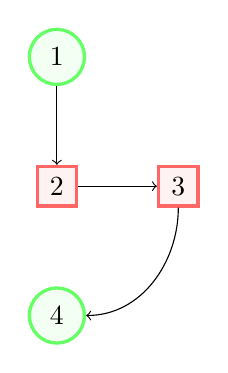
\begin{tikzpicture}[
roundnode/.style={circle, draw=green!60, fill=green!5, very thick, minimum size=7mm},
squarednode/.style={rectangle, draw=red!60, fill=red!5, very thick, minimum size=5mm},
]
%Nodes
\node[squarednode]      (maintopic)                              {2};
\node[roundnode]        (uppercircle)       [above=of maintopic] {1};
\node[squarednode]      (rightsquare)       [right=of maintopic] {3};
\node[roundnode]        (lowercircle)       [below=of maintopic] {4};

%Lines
\draw[->] (uppercircle.south) -- (maintopic.north);
\draw[->] (maintopic.east) -- (rightsquare.west);
\draw[->] (rightsquare.south) .. controls +(down:7mm) and +(right:7mm) .. (lowercircle.east);

\end{tikzpicture}

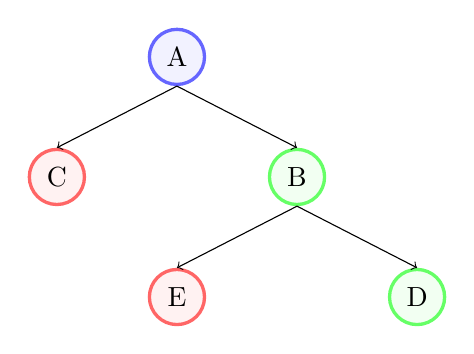
\begin{tikzpicture}[
yesnode/.style={circle, draw=green!60, fill=green!5, very thick, minimum size=7mm},
nonode/.style={circle, draw=red!60, fill=red!5, very thick, minimum size=7mm},
startnode/.style={circle, draw=blue!60, fill=blue!5, very thick, minimum size=7mm},
]
\node[startnode]          (start)                                           {A};
\node[yesnode]            (firstyes)        [below right=of start]          {B};
\node[nonode]             (firstno)         [below left=of start]           {C};
\node[yesnode]            (secondyes)       [below right=of firstyes]       {D};
\node[nonode]             (secondno)        [below left=of firstyes]        {E};

\draw[->] (start.south) -- (firstyes.north);
\draw[->] (start.south) -- (firstno.north);
\draw[->] (firstyes.south) -- (secondyes.north);
\draw[->] (firstyes.south) -- (secondno.north);

\end{tikzpicture}
\newpage

\section{tikzplotlib}
Now to the really cool part: directly importing your matplotlib figures from whatever project you are working on as .tex file, providing high quality and easy editing.

% This file was created with tikzplotlib v0.10.1.
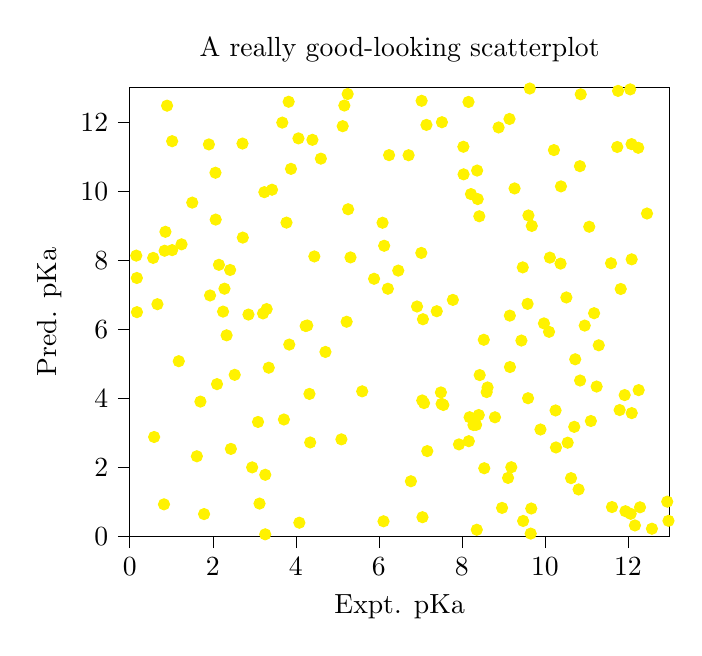
\begin{tikzpicture}

\definecolor{darkgray176}{RGB}{176,176,176}
\definecolor{royalblue}{RGB}{65,105,225}

\begin{axis}[
tick align=outside,
tick pos=left,
title={A really good-looking scatterplot},
x grid style={darkgray176},
xlabel={Expt. pKa},
xmin=0, xmax=13,
xtick style={color=black},
y grid style={darkgray176},
ylabel={Pred. pKa},
ymin=0, ymax=13,
ytick style={color=black}
]
\addplot [draw=yellow, fill=yellow, mark=*, only marks]
table{%
x  y
5.24929707001315 12.8217334657533
9.8934671294092 3.09367268519743
12.088613853441 11.36891005865
3.82795084342127 12.5975305618489
10.9603179274238 6.10733871272123
13.4886433604514 2.07523790991018
2.28088841396565 13.6687853268893
5.22460671597504 6.21807960282779
10.2181213211852 11.1956686597487
12.2490043587356 11.2623389744804
13.3896230872677 11.5080557076998
12.0924015922019 3.56898127203076
4.08536021932559 0.390632074307994
13.9652674501561 0.344354070521574
11.1081547865882 3.3396386472473
2.41786319296919 7.71980233331204
11.616507932933 0.845307780590133
12.0553639155081 12.9566596937033
4.32865156261594 4.12579878132122
3.34842800994376 4.88572978993864
0.156940425719107 8.1357551288475
13.2465600969477 5.35879466225211
1.93449982469559 6.98065711272478
8.35983567359608 0.186375847670712
0.898882762044815 12.4843962403702
6.77270950025722 1.59305131362135
8.96875468009169 0.820435321245501
13.0452940119879 3.97574981692323
10.3724340410164 13.5174726991782
2.24770697586361 6.51232866279264
8.88553993631785 11.8518148402061
11.5937095430963 7.91413333774291
8.16014353931699 12.591821904661
10.7076078489986 3.17081431466792
10.3872555556662 10.1431585911135
11.7436378527781 11.2861837741586
10.5495020095724 2.71089989280166
3.12592305988243 0.945830014840155
10.1205256017286 8.07769716010449
1.8960752506198 13.0357745528942
4.3465527497766 2.71736706097596
0.84027773358363 8.27733102028831
11.9223761887909 4.09178989471282
2.85954379820594 6.42638999080738
4.06366008453775 11.5352129501309
3.21030941490761 6.45993584662953
10.8637553645055 12.813138752961
8.16782839055733 2.75438482567601
9.94535454017241 13.5153676644165
11.2472001804883 4.33965381795079
7.49543433216588 4.16929681780609
12.9778813491154 0.445727553930706
6.46816138188285 7.70137141260318
8.04174130511345 10.4926095702879
13.8963921557373 9.16749300467453
0.666245640489301 6.72708542027417
5.3177111532151 8.08375497423196
7.35677792194185 13.8362326885666
5.12973941916247 11.8893271193073
3.2645349764478 1.78077590694594
13.645928248331 9.71722044369142
8.42982134555183 4.6718814999084
2.14792434963207 7.86891344954593
8.38188068072462 9.77557390489559
8.21927276792341 9.92010240148258
2.7159537869547 11.3852667381611
13.8834324001892 12.5624969334386
8.42067526420961 9.27679563942686
12.4602031940921 9.35668804062263
1.70165938154606 3.90302701018821
11.8009020593103 3.65810555994664
9.60367196400472 9.30001282480439
7.0895867721311 3.85919396969611
2.28169435134981 7.1768805719923
3.26296411632062 0.054091989674
0.586965647451699 2.87681267415632
1.79020862470402 0.641103348752618
8.79800604231165 3.4477344347755
6.9205602415786 6.66061592471873
4.27627745477404 6.10926644312966
7.80341973615746 13.3825904163393
9.97777242120772 6.17024546077358
3.09004192888517 3.31265072038647
11.7630664897573 12.9125632976802
4.44659654406419 8.11209739308609
9.19127298073439 1.9994236792016
1.2471954362621 8.46294317618203
1.90623083489194 11.3603261349969
3.71351442780802 3.38361420056029
1.50561678630388 9.67284927871408
3.67444435241798 11.9927292593019
2.07021464379701 9.18053626340536
10.1001730725636 5.92594255672281
12.9477548059611 1.00144720087419
9.47622505878278 0.441640013321538
1.18053673149983 5.07437716583991
13.6667517588662 8.07192896259646
12.0671012006571 0.648695065909256
8.18659414276186 3.45013906078466
6.21794720850863 7.17558162418119
7.39579846230309 6.5234293561675
1.61647789381589 2.31729077229499
7.51226874516592 3.83758520036125
4.23722798925622 6.09475581244071
9.63672534911745 12.9809292863234
7.02347760049269 8.21383683438021
8.38600406868717 13.7111788630795
9.58360207656137 6.73680053568777
6.08939026865372 9.08887695289127
0.564149310475921 8.06955361514275
3.8835707354671 10.6515436695329
5.88540383074751 7.46421318377468
12.578886939461 0.216614102958955
8.40771785619595 3.51321455845443
9.43456964494468 5.6726990935827
7.01777412319909 13.9420827636997
3.77558055688987 9.09261851395374
8.61970549162554 4.31265607374211
1.02115734605509 11.4542973521258
6.24687857906809 11.0496601062616
5.26063164365995 9.48020501440538
10.3782261209527 7.90406917692248
5.1690806331258 12.4883758768482
4.71414607563397 5.3429638220904
9.11311503293516 1.69005343360249
4.60356426304159 10.9479010998543
10.8441215689377 10.7299159766811
2.06462730551192 10.5391872998252
9.6587861834609 0.075258855378507
13.3407651594743 9.05069569160694
11.8273435916002 7.16847209614724
7.04575515513619 3.93595361623967
11.1856975914484 6.46607839579155
7.14728330738621 11.9262311623506
9.46743125539774 7.79475376889548
7.55464237252031 3.80490256924797
6.11297008959261 0.432210417327528
0.171218053515666 7.48734634429964
10.7309170858008 5.12988393823685
2.94834477452284 1.99524591588239
0.85930705066194 8.82666801831454
1.02046022738941 8.29520634915787
7.05183691008791 0.550746634070793
13.5027098081865 0.0127174705122766
8.52842347663388 5.69540547930794
12.2921687564439 0.838021409295172
5.09818529054181 2.80767461214911
8.59788495349149 4.17837257556842
7.78345299599173 6.85184410324354
8.36811399330373 10.602255196651
7.51993207436893 12.0042849756728
3.24242791306263 9.9760416535522
10.6304300366908 1.68324278603033
4.80476779064928 13.7246338954518
2.7230585185311 8.65847803800689
9.14753526560846 12.0983970233293
11.0691119847282 8.97249067637348
10.2578711993992 3.64621470823982
2.43595750662598 2.53116838028406
3.84250720947712 5.55619593211282
7.93031705675253 2.66159334048667
2.33299729793264 5.824684184077
12.2595004344554 4.23562744540722
8.34297021029558 3.22750258482306
9.2703009871512 10.0840473831615
12.0908008691058 8.02812678012834
9.15618737716214 6.39604773835402
6.12878010459472 8.42187785241828
7.06252049649919 6.29128978170337
8.54013952964141 1.97054513207991
9.15943296881629 4.90531827065186
4.40021058650117 11.4933213655747
4.23940607905771 13.8762259999774
13.0593813917432 4.47337040972132
13.1229619900937 8.19350104762391
9.68479602036549 8.99688852113284
7.03078461799666 12.6249006388548
8.27873975661607 3.22469048362927
0.824422089437975 0.923784321760886
11.940695540679 0.724512521931888
3.42686765417152 10.0466006077156
6.71745417919585 11.0468558046065
5.59912299792661 4.20036123515906
8.03657383026527 11.2926582407794
13.5018761205147 3.97327480276887
12.1696063981383 0.312041342121409
10.8124866920533 1.35500105968403
7.12117292517335 13.2773946177341
2.1018873132504 4.40944543052692
9.67196793772533 0.802390511125864
10.2677641271599 2.57307187231056
9.59511419847698 4.00057106844572
10.8487987535536 4.51410598802623
11.3898198252803 13.6632891263078
3.29785640597247 6.58542096374906
11.2980525730174 5.53540725679763
7.16738916267359 2.4673308671584
0.173172485610358 6.49663287893234
10.5178111263796 6.92267280841331
2.52833308094491 4.67915160927199
};
\end{axis}

\end{tikzpicture}

\vspace{5mm}

\begin{figure}
    \centering
    % This file was created with tikzplotlib v0.10.1.
\begin{scaletikzpicturetowidth}{\textwidth}
\begin{tikzpicture}[scale=\tikzscale]

\definecolor{darkgray176}{RGB}{176,176,176}
\definecolor{forestgreen}{RGB}{34,139,34}
\definecolor{lightgray204}{RGB}{204,204,204}
\definecolor{orangered}{RGB}{255,69,0}

\begin{axis}[
legend cell align={left},
legend style={fill opacity=0.8, draw opacity=1, text opacity=1, draw=lightgray204},
tick align=outside,
tick pos=left,
x grid style={darkgray176},
xlabel={Age},
xmin=-0.3, xmax=3.55,
xtick style={color=black},
xtick={0.125,1.125,2.125,3.125},
xticklabel style={rotate=60.0},
xticklabels={18-25,26-39,40-49,50-65},
y grid style={darkgray176},
ylabel={Amount of problems},
ymin=0, ymax=1034.25,
ytick style={color=black}
]
\draw[draw=none,fill=orangered] (axis cs:-0.125,0) rectangle (axis cs:0.125,911);
\draw[draw=none,fill=orangered] (axis cs:0.875,0) rectangle (axis cs:1.125,225);
\draw[draw=none,fill=orangered] (axis cs:1.875,0) rectangle (axis cs:2.125,985);
\draw[draw=none,fill=orangered] (axis cs:2.875,0) rectangle (axis cs:3.125,93);
\draw[draw=none,fill=forestgreen] (axis cs:0.125,0) rectangle (axis cs:0.375,438);
\draw[draw=none,fill=forestgreen] (axis cs:1.125,0) rectangle (axis cs:1.375,957);
\draw[draw=none,fill=forestgreen] (axis cs:2.125,0) rectangle (axis cs:2.375,502);
\draw[draw=none,fill=forestgreen] (axis cs:3.125,0) rectangle (axis cs:3.375,412);
\end{axis}

\end{tikzpicture}
\end{scaletikzpicturetowidth}

    \caption{What a nice bar graph! Just look at that beautiful thing, sitting right there in the center}
    \label{fig:bar}
\end{figure}


\end{document}
